\subsection{Ego4D}
\begin{frame}[allowframebreaks]{Ego4D: New Large-Scale Video Dataset}
    \textbf{Ego4D} is a large-scale dataset designed to advance the understanding of egocentric (first-person) video. It consists of over 3,670 hours of egocentric video footage captured using head-mounted cameras.

    \begin{itemize}
        \item \textbf{Long Videos:} Each video ranges from \textit{1 to 10 hours} in length.
        \item \textbf{Diversity:} Data collected by \textit{14 teams} across \textit{9 countries}, \textit{74 locations}, involving \textit{931 unique camera wearers}.
        \item \textbf{Natural-Language Narrations:} Contains \textit{3.85 million} sentences of narrations.
        \item \textbf{Rich Annotations:} Supports \textit{5 different tasks}:
        \begin{itemize}
            \setlength{\itemsep}{-0.5em}
            \item Episodic Memory
            \item Hands and Objects
            \item Audio-Video Diarization
            \item Social Interactions
            \item Forecasting
        \end{itemize}
    \end{itemize}
\framebreak
    \textbf{Key Features of Ego4D:}
    \begin{itemize}
        \item \textbf{First-Person Perspective:} Captures videos from the viewpoint of the person wearing the camera, providing a unique perspective on human activities.
        \item \textbf{Large Scale:} 3,670 hours of video data, making it one of the largest datasets for egocentric video understanding.
        \item \textbf{Diverse Activities and Participants:} Wide range of activities and a large, varied set of camera wearers, reflecting real-world scenarios.
        \item \textbf{Comprehensive Annotations:} Natural-language narrations and support for multiple tasks enable comprehensive model training and evaluation.
    \end{itemize}
\framebreak
    \begin{figure}
        \centering
        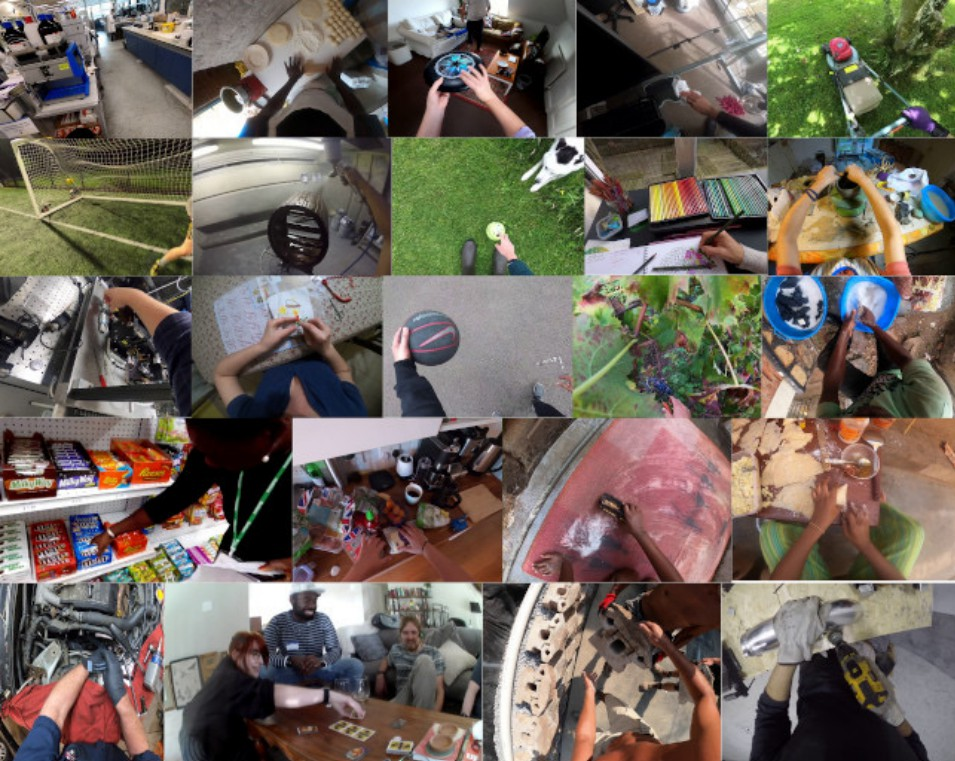
\includegraphics[width=1\textwidth,height=0.9\textheight,keepaspectratio]{images/video/slide_42_1_img.jpg}
    \end{figure}
\end{frame}
    